\documentclass[paper=a4, fontsize=11pt]{scrartcl} % A4 paper and 11pt font size

\usepackage{amsmath,amsfonts,amsthm} % Math packages
\usepackage[english]{babel}
\usepackage{graphicx}

\title{Data Mining Assignment 3}
\author{Yulong Yang\\ netid: \textit{yy231}} % Your name


\date{\normalsize\today} % Today's date or a custom date
\begin{document}

\maketitle % Print the title

%%%%%%%%%%%%%%%%
%%%%% Question 1 %%%%%
%%%%%%%%%%%%%%%%
\section*{Question 1}

\subsection*{a}

As we have 5 unique items, the theoretical maximum for number of rules is given by this formula: $3^5 - 2^{5+1}+1=180$.

\subsection*{b}

Transactions from the table has at most 4 items, therefore the maximum size possible is 4.

\subsection*{c}

The answer is the 3-item combinations chose from 5 different items: $5!/3!=10$.

\subsection*{d} 

\{D, E\}.

\subsection*{e}

\{A,C\} and \{C,A\}. 

%%%%%%%%%%%%%%%%
%%%%% Question 2 %%%%%
%%%%%%%%%%%%%%%%
\section*{Question 2}

Please find the lattice drawing and labels in the next page. For each node, the character in red is the label.

%%%%%%%%%%%%%%%%
%%%%% Question 3 %%%%%
%%%%%%%%%%%%%%%%
\section*{Question 3}

\subsection*{a}

Data set 2 will produce more because it contains more itemsets with support surpasses $minsup$, which is indicated by those rectangles.

\subsection*{b}

In the graph, each dark-color square indicates one closed frequent 200-itemset, therefore the answer is 5.

\subsection*{c}

Data set 2 has the longer frequent itemset because it has more items appear together in same transactions around transactions 2000-4000 than anyone from data set 2.

\subsection*{d}

If we look at the vertical edge of each data set, there are rectangles in data set 2 having longer length than squares in data set 1. Such vertical length indicates the number of transactions those items appear together. Therefore, data set 2 produces the high support.

\subsection*{e}

Still data set 2, as it has more frequent itemsets and most of them are not immediate supersets of each other.

%%%%%%%%%%%%%%%%
%%%%% Question 4 %%%%%
%%%%%%%%%%%%%%%%
\section*{Question 4}

The sketch of five questions is showing together as below, and followed by text answers separately for each question. In the graph, ``+" indicates a centroid.

\begin{figure}[htbp]
\begin{center}
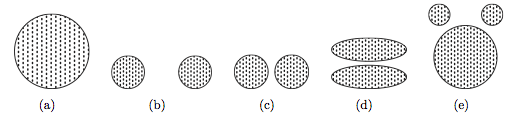
\includegraphics[width=\textwidth]{hw3pic1}
\caption{Sketch of K-means}
\label{hw3pic1}
\end{center}
\end{figure}

\subsection*{a}

There could be arbitrarily number of possible ways of partitioning the data, as they are uniformly distributed in the area. The SSE of every way would be the same regardless the position of two centroids, therefore all solutions are global minimum.

\subsection*{b}

There could be also arbitrarily ways of partitioning the dataset. Because either of the circle could be portioned into two, and the ways of partitioning it is arbitrary. Again, all solutions are global minimum because distances are minimized.

\subsection*{c}

There could be only one solution for the clustering as shown in the graph and it is the global minimum. 

\subsection*{d}

There could be two ways of splitting it, either the one shown above, or splitting vertically in the middle. The vertical one is global while the horizontal split is local, because in the way of latter split, its distance is larger than former. 

\subsection*{e}

There will only be one global minimum solution, which is shown above.

%%%%%%%%%%%%%%%%
%%%%% Question 5 %%%%%
%%%%%%%%%%%%%%%%
\section*{Question 5}

Please find the dendrograms below.

\end{document}